\documentclass[conference]{IEEEtran}
\usepackage{amsmath,amssymb}
\usepackage{graphicx}
\usepackage{booktabs}
\usepackage{adjustbox}
\usepackage{tikz}
\usetikzlibrary{arrows.meta,positioning,fit}
\usepackage{url}
\usepackage[hidelinks]{hyperref}
\graphicspath{{figures/}}
\newcommand{\eg}{e.g.\ }

\begin{document}

\title{Behaviour Cloning a Mobile Manipulator with a Recurrent Velocity-Field Policy}

\author{\IEEEauthorblockN{COMP0245 Group [number] --- [Member names]}
\IEEEauthorblockA{University College London}}

\maketitle

\begin{abstract}
We clone the template expert that drives a four-wheeled base and a 7-DoF arm to a 3-D target. A single
GRU maps base pose, joint angles and target to wheel commands, a stop decision, and a $7{\times}3$ matrix
$M$; the arm's desired joint velocity is $M e$ for end-effector error $e$, tracked by a joint PD layer.
Labels come from recorded states only: wheel commands, finite-difference joint velocities, and a stop
time read off the wheel commands. On 300 fresh scenes collected after freezing, the policy reaches the
1\,cm target in 98.7\% of runs (expert 97.7\%, $p=0.55$), holds it as well as the expert, recovers from
base pushes that defeat the expert (56/60 vs 38/60), and runs in 87\,$\mu$s per 1\,kHz step. Ablations show
that the action representation decides whether cloning works at all: direct torque regression succeeds
in 2/208 validation scenes.
\end{abstract}

\section{Introduction}
The template expert parks the base on the ray from the world origin to the target, at a height-dependent
standoff, then reaches with differential inverse kinematics (IK) and a joint PD law with gravity
compensation. Our task is to learn a regressor from the measured state $(\texttt{base\_pos},
\texttt{base\_bearing}, \texttt{q\_mes}, \texttt{qd\_mes})$ and \texttt{TARGET\_EE\_POS} to
\texttt{wheel\_cmds} (4) and \texttt{torque\_arm} (7) by behaviour cloning (BC)~\cite{pomerleau1989}:
supervised learning on expert trajectories.

\textbf{Assumptions and constraints.} (i) Simulation only (PyBullet, 1\,kHz). (ii) The learner may use the
listed measurements, the target, and the robot's kinematic model to compute the end-effector position;
it may \emph{not} read the expert's internal variables (phase, $q_\text{des}$, navigation state) or call
the expert at run time. We enforce this in code: learned rollouts abort if the expert module is
imported. (iii) Success follows the template's \texttt{check\_stop}: base finished, error $<1$\,cm,
$t>8$\,s; episodes end at 40\,s.

Plain BC suffers from compounding error: small action errors move the robot to states absent from the
demonstrations~\cite{ross2011}. Our design choices aim at a representation in which such errors are
self-correcting, and each choice is backed by an ablation (Table~\ref{tab:ablation}).

\section{Methodology}

\subsection{Expert data}
We sample 1500 scenes (target $x,y\in[-1.6,1.6]$\,m, $z\in[0.1,1.3]$\,m; base start $\pm0.6$\,m, any
heading; arm start $\pm0.15$\,rad around the template posture) and run the expert headless at 1\,kHz,
recording inputs, actions and end-effector position. We keep the 1391 successful runs and split them by
whole trajectory (seed 42) into 973/208/210 for training, validation and a development test set;
splitting by frame would leak near-identical neighbouring frames. Normalisation uses training data only.
The learning curve (Fig.~\ref{fig:lc}) shows how much data is needed: success rises from 157/208 with 97
trajectories to 207/208 with 973, and the three validation losses fall monotonically.

\subsection{What to imitate: labels from states}
Expert torques mix gravity, dynamics and the expert's own PD reaction, so they are a poor target for a
regressor whose errors feed back through the dynamics. We therefore imitate \emph{observations}, in the
spirit of BC from observation~\cite{torabi2018}:
\begin{itemize}
\item \textbf{Wheels:} the recorded wheel commands (already kinematic).
\item \textbf{Arm:} desired joint velocity $v_k=(q_{t+10}-q_{t-10})/20$\,ms, a central difference of
recorded joint angles.
\item \textbf{Stop:} $c_k=\mathbb 1[t\ge t_\text{stop}]$, where $t_\text{stop}$ is the first step after which
every recorded wheel command stays zero. It needs only the recorded actions, yet matched the expert's
internal ``navigation done'' time on all 60 trajectories we checked.
\item \textbf{Parking pose:} the recorded base pose at $t_\text{stop}$, one sample per trajectory.
\end{itemize}

\subsection{Policy}
Fig.~\ref{fig:arch} shows the policy. Every 10\,ms a GRU~\cite{cho2014} (128 hidden units) reads 18
features in the base frame: target position and distance, the parking pose predicted by a small MLP
from the target, the end-effector error $e$, and the 7 joint angles. It outputs 4 wheel commands, a
stop logit $s_k$, and $M\in\mathbb R^{7\times3}$.

\begin{figure}[t]
\centering
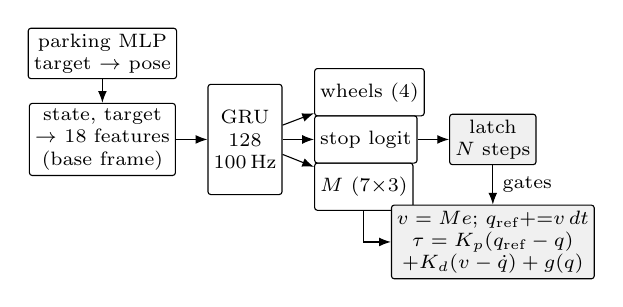
\begin{tikzpicture}[font=\scriptsize, node distance=3mm and 4mm,
  box/.style={draw, rounded corners=1pt, align=center, inner sep=2pt, minimum height=6mm},
  fixed/.style={box, fill=gray!12}, arr/.style={-{Latex[length=1.5mm]}}]
\node[box] (in) {state, target\\$\to$ 18 features\\(base frame)};
\node[box, above=of in] (park) {parking MLP\\target $\to$ pose};
\node[box, right=of in, minimum height=14mm] (gru) {GRU\\128\\100\,Hz};
\node[box, right=of gru, yshift=6mm] (w) {wheels (4)};
\node[box, right=of gru] (s) {stop logit};
\node[box, right=of gru, yshift=-6mm] (m) {$M$ ($7{\times}3$)};
\node[fixed, right=of s] (latch) {latch\\$N$ steps};
\node[fixed, below=5mm of latch] (pd) {$v=Me$; $q_\text{ref}{+}{=}v\,dt$\\$\tau=K_p(q_\text{ref}-q)$\\$+K_d(v-\dot q)+g(q)$};
\draw[arr] (park) -- (in); \draw[arr] (in) -- (gru);
\draw[arr] (gru) -- (w); \draw[arr] (gru) -- (s); \draw[arr] (gru) -- (m);
\draw[arr] (s) -- (latch); \draw[arr] (m.south) |- (pd.west);
\draw[arr] (latch) -- node[right]{gates} (pd);
\end{tikzpicture}
\caption{Policy. White: learned from demonstrations. Grey: fixed structure. Before the latch the
wheels follow the GRU and the arm holds its start pose; after it the wheels stop and the arm reaches.
The PD layer runs at 1\,kHz.}
\label{fig:arch}
\end{figure}

\textbf{Velocity field $v=Me$.} The arm's desired joint velocity is $v=Me$. This guarantees $v=0$ at
$e=0$, so the arm stops at the target, and $M$ has the shape of a damped least-squares IK map
$J^\top(JJ^\top+\lambda^2I)^{-1}$ that the network learns without a Jacobian. Because $e$ is recomputed
every 1\,ms from the current state, a model error changes the \emph{direction} of approach but not the
fixed point: the loop corrects its own mistakes instead of compounding them. A reference
$q_\text{ref}\leftarrow\text{clip}(q_\text{ref}+v\,dt,\;q\pm\text{lead})$ is tracked by
$\tau=K_p(q_\text{ref}-q)+K_d(v-\dot q)+g(q)$; this is how the robot actually receives
\texttt{torque\_arm}. Regressing torques directly instead reaches 2/208 on validation
(Table~\ref{tab:ablation}): small errors in a gravity-dominated signal diverge in closed loop.

\textbf{Memory and an explicit stop.} A single frame cannot distinguish ``slowing down near the parking
pose'' from ``parked''. Four single-frame MLPs reach 195/208; a GRU whose phases must emerge from the
hidden state alone (no stop output) reaches only 88/208, because a regressed wheel speed approaches zero
without ever committing to stop. We therefore add a stop logit trained with binary cross-entropy and
latch it after $N$ consecutive positive outputs; the latch makes the decision monotonic.

\textbf{Learned parking pose (variant B) vs.\ a hand-made feature (v3).} The parking pose is not
translation invariant: it lies on the origin--target ray. Our baseline v3 encodes this with a world-bearing
feature $\text{atan2}(t_y,t_x)-\psi$ copied from the expert's code. Variant B instead learns it: an MLP
(2$\times$128 ReLU, 17,540 parameters) maps the target to the parking pose, which enters the GRU as
base-frame coordinates. This removes the last expert formula from the inputs.

\textbf{Why these features.} The expert's base law uses only relative quantities (distance, heading and
yaw errors), so all features are expressed in the base frame and angles as $\sin/\cos$. Joint velocities
are omitted: they are noisy and the PD layer already uses them.

\subsection{Training}
The loss is $L=L_\text{wheel}+L_\text{arm}+L_\text{stop}$: MSE on normalised wheel commands, MSE on
$(Me-v)/\sigma_v$ over frames after $t_\text{stop}$ only (the arm is held before), and BCE on $s_k$.
We use Adam ($10^{-3}$), batches of 32 whole trajectories with masking, full back-propagation through
time with gradient clipping at 1, and early stopping on validation loss (patience 8, at most 80 epochs).
Although the arm loss covers only post-stop frames, its gradient flows back through the hidden state, so
the GRU can store during navigation what the arm needs later. Variant B trains in 31\,min on a CPU
(best epoch 78). The run-time forward pass is NumPy; it matches PyTorch to $7.7\times10^{-6}$.

\textbf{Hyperparameters chosen on validation.} The latch length $N$ is chosen open-loop on validation
sequences (smallest mean offset to $t_\text{stop}$; $N=1$ for B). The gains $(K_p,K_d,\text{lead})$ cannot
be learned with the network (the loss does not depend on them, and closed-loop success is not
differentiable through the simulator), so we grid-search $\{50,100,200\}\times\{10,30\}\times\{0.1,0.2\}$
in closed loop on all 208 validation scenes, with a rule fixed beforehand: most successes, then shortest
mean time, then fewest torque-clipped steps. With 12 cheap points and a flat landscape (10 of 12 give
206--207 for B), grid search is preferable to Bayesian optimisation. B chose 200/30/0.2, v3 100/10/0.1.

\section{Experiments and Results}

\subsection{Protocol}
During development the original test split was used three times and variant B was designed after
inspecting its failures, so it is no longer unbiased. We therefore fixed a protocol before seeing
results: retrain both models, choose gains on validation, check that development numbers reproduce
(within $\pm3$ scenes: 204 vs 205 for v3, 208 vs 206 for B), \emph{freeze}, then collect 300 new scenes
(seed 2026) and evaluate once. The fresh set is not filtered by expert success, which removes the
selection bias of testing only on scenes the expert solved. All controllers run on identical scenes,
so we compare them with the exact McNemar test on discordant pairs and report Wilson 95\% intervals.

\subsection{Accuracy}
Table~\ref{tab:main} gives the main results. B reaches 296/300 (98.7\%); the expert reaches 293/300.
The difference is not significant ($p=0.55$), so we claim parity, not superiority. B also solves all 14
scenes where the expert failed during collection, although no such scene was used for training. Its four failures are three latches that never fire and one arm that stops 6\,cm short; both
are consistent with covariate shift~\cite{ross2011}: the policy reaches states that are rare in the
demonstrations.

The template's success test only checks the \emph{first} entry into 1\,cm. To test accuracy beyond that
instant we continue each successful run for 2\,s. B and the expert stay within 1\,cm in 286 runs each
and settle to a median 0.6\,mm. v3 stays in only 171 of its 289 successes ($p=3\times10^{-28}$ vs B).
Fig.~\ref{fig:hold} shows why: v3 oscillates around the target (dominant frequency 0.5--1.5\,Hz).

\begin{table}[t]
\centering\footnotesize
\caption{Fresh test set (300 scenes, seed 2026, evaluated once after freezing)}
\label{tab:main}
\begin{adjustbox}{max width=\columnwidth}\begin{tabular}{@{}lccc@{}}
\toprule
 & \textbf{B-FK (ours)} & B, URDF FK & Expert \\
\midrule
1 cm success / 300 & \textbf{288} & 296 & 293 \\
\quad rate (\%) & 96.0 & 98.7 & 97.7 \\
\quad 95\% Wilson CI & 93.1--97.7 & 96.6--99.5 & 95.3--98.9 \\
Held $<$1 cm for 2 s & 277 & 286 & 286 \\
Mean time to success (s) & 9.19 & 9.28 & 9.29 \\
Compute per 1 kHz step ($\mu$s) & 342 & 87 & 82 \\
Learned parameters & 346,017 & 77,726 & -- \\
Robot model in the policy & none & FK, $g(q)$ & FK, IK, $g(q)$ \\
\midrule
\multicolumn{4}{@{}l@{}}{Exact McNemar (discordant pairs): B-FK vs expert 6/11, $p=0.33$;} \\
\multicolumn{4}{@{}l@{}}{B-FK vs B 2/10, $p=0.04$. Held: B-FK vs expert 7/16, $p=0.09$.} \\
\bottomrule
\end{tabular}
\end{adjustbox}
\end{table}

\begin{figure}[t]
\centering
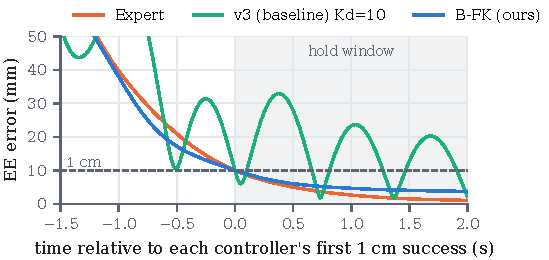
\includegraphics[width=\columnwidth]{hold_trace.pdf}
\caption{End-effector error in scene 2026\_0008, aligned at each controller's first 1\,cm success.
B and the expert converge; v3 with its chosen $K_d=10$ oscillates.}
\label{fig:hold}
\end{figure}

\subsection{Ablations: what makes cloning work}
Table~\ref{tab:ablation} collects the ablations.
\begin{itemize}
\item \textbf{Action representation} decides feasibility: direct torque regression reaches 2/208;
the velocity field reaches 207.
\item \textbf{Memory and the stop decision:} without the stop output the GRU reaches 88/208.
\item \textbf{Learned vs.\ hand-made parking information:} 207 vs 205 on validation and 296 vs 289 on the
fresh test ($p=0.09$). Learning the pose is at least as good as copying the expert's formula.
\item \textbf{Gravity model:} removing $g(q)$ leaves B unchanged at the chosen gains (207/208). The
integrated reference acts as an integral term, and $K_p\cdot\text{lead}=40$\,N\,m exceeds the shoulder's
gravity load (median recorded torque 17.7\,N\,m). At 50/30/0.1 (5\,N\,m) the arm sags (57/208). The
robot's dynamic model is therefore not required.
\item \textbf{Damping, a lesson about the metric:} swapping gains moves the oscillation with $K_d$:
v3 with $K_d=30$ holds in 278/289 runs, B with $K_d=10$ in only 144/296. Neither change alters the 1\,cm
success count. Our selection rule broke ties by speed, and a first-entry success test cannot see the
missing damping, so it favoured the under-damped gains for v3. We found this on the test set, so we
report it as a diagnosis and did not retune v3; the fix is to include holding in the selection rule.
\item \textbf{Seeds:} GRU seeds 1 and 2 reach 207 and 208, so the result is not a lucky initialisation.
\end{itemize}

\begin{table}[t]
\centering\footnotesize
\caption{Ablations (validation set, 208 scenes, unless noted)}
\label{tab:ablation}
\begin{adjustbox}{max width=\columnwidth}\begin{tabular}{@{}lcl@{}}
\toprule
Variant & Success / 208 & Note \\
\midrule
\multicolumn{3}{@{}l}{\emph{Development runs (same validation set)}} \\
Four MLPs, single-frame input & 195 & no memory \\
GRU without stop head (v2) & 88 & never stops \\
GRU, direct torque output & 2 & diverges \\
\multicolumn{3}{@{}l}{\emph{Final run}} \\
v3: hand-made bearing feature & 205 & gains 100/10/0.1 \\
\textbf{B}: learned parking pose & \textbf{207} & gains 200/30/0.2 \\
B, GRU seeds 1 / 2 & 207 / 208 & seed spread \\
B, gains: other 11 combinations & 193--207 & gain sensitivity \\
B without $g(q)$ & 207 & chosen gains \\
B without $g(q)$, gains 50/30/0.1 & 57 & with $g(q)$: 203 \\
\midrule
\multicolumn{3}{@{}l}{\emph{Hold test, fresh set: held $<$1 cm for 2 s / successes}} \\
v3, Kd=10 (own gains) & 171 / 289 & \\
v3 with Kd=30 & 278 / 289 & \\
B, Kd=30 (own gains) & 286 / 296 & \\
B with Kd=10 & 144 / 296 & \\
\bottomrule
\end{tabular}
\end{adjustbox}
\end{table}

\subsection{Robustness and generalisation}
Fig.~\ref{fig:cond} shows perturbed and out-of-distribution (OOD) scenes; B and the expert see identical
perturbations.
\begin{itemize}
\item \textbf{Noise, weak actuators, end-effector push:} B scores 59/60 in all four conditions. Its one
failure is the same scene as without perturbation, so the closed loop absorbs these disturbances.
\item \textbf{Base push} (20\,N for 0.2\,s): B 56/60 vs expert 38/60 ($p=4\times10^{-5}$). The wheels have
almost no lateral friction, so the push slides the base about a metre. The expert's state machine does
not recover before its 25\,s time-out; the GRU re-plans from the current pose every 10\,ms.
\item \textbf{High targets:} B 40/40 vs expert 15/40. The expert projects targets onto a 0.85\,m reach
sphere and stops 1.8--5.8\,cm short.
\end{itemize}
Both results show that BC copies the demonstrated \emph{behaviour}, not the expert's hard-coded limits,
which never appear in the data. Low targets ($z<0.1$\,m) remain hard for both controllers (29 vs 30 of
40) because of joint limits near the floor.

\begin{figure}[t]
\centering
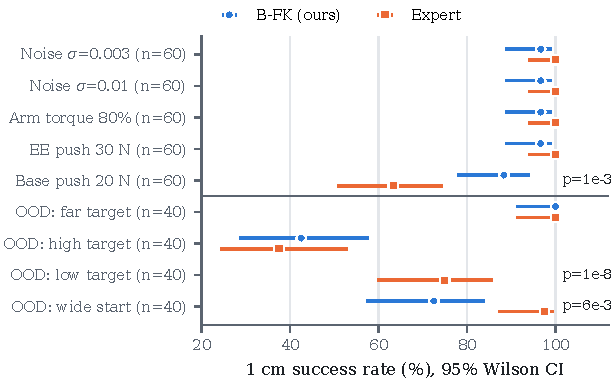
\includegraphics[width=\columnwidth]{conditions.pdf}
\caption{Robustness (60 fresh scenes) and OOD families (40 scenes each). $p$: exact McNemar, shown
when $<0.05$.}
\label{fig:cond}
\end{figure}

\subsection{Efficiency}
The policy has 77,726 parameters (616\,KiB) and needs 87\,$\mu$s per 1\,kHz control step, including
features, a GRU update every tenth step and the PD layer; the expert's IK needs 82\,$\mu$s. Training
takes 31\,min on a CPU. For data efficiency, Fig.~\ref{fig:lc} shows that with little data the
\emph{base} fails first: at 97 trajectories half the failures never latch, and at 243--486 the base parks
where the arm cannot reach (median parking offset 10.8 and 8.7\,cm vs 7.5\,cm with all data). At 243 trajectories and above, most
failures come from the base rather than from the arm velocity field.

\begin{figure}[t]
\centering
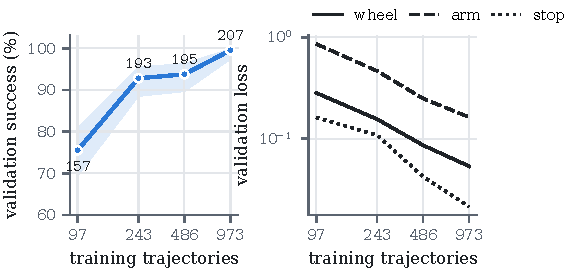
\includegraphics[width=\columnwidth]{learning_curve.pdf}
\caption{Learning curve: nested subsets of the training trajectories, evaluated in closed loop on the 208
validation scenes (shaded: Wilson 95\% CI).}
\label{fig:lc}
\end{figure}

\section{Conclusion}
A recurrent policy that outputs a velocity field rather than torques, with an explicit latched stop
decision and a learned parking pose, clones the expert to parity on fresh scenes, holds the target as
well as the expert, and is more robust to base disturbances. The ablations show that in BC the choice of
\emph{what} to imitate and \emph{how} to act matters more than accuracy on recorded data.

\textbf{Limitations.} (i) Training sees only expert states; no DAgger-style aggregation~\cite{ross2011}
corrects the rare missed latches. (ii) The PD layer, the park-then-reach structure and the latch are fixed,
and forward kinematics uses the robot model. (iii) The template's first-entry success test hides poor
damping, which biased our gain selection. (iv) Robustness and OOD tests use 40--60 scenes and one
perturbation level; only the GRU seed was varied.

\textbf{Improvements.} Aggregate policy roll-outs relabelled with the expert (DAgger); learn a residual
torque on top of the PD layer; select gains and report success with a holding criterion; sweep
perturbation strength.

\begin{thebibliography}{9}
\bibitem{pomerleau1989} D.~A. Pomerleau, ``ALVINN: An autonomous land vehicle in a neural network,'' in
\emph{NeurIPS}, 1989.
\bibitem{ross2011} S.~Ross, G.~Gordon, and D.~Bagnell, ``A reduction of imitation learning and structured
prediction to no-regret online learning,'' in \emph{AISTATS}, 2011.
\bibitem{torabi2018} F.~Torabi, G.~Warnell, and P.~Stone, ``Behavioral cloning from observation,'' in
\emph{IJCAI}, 2018.
\bibitem{cho2014} K.~Cho \emph{et al.}, ``Learning phrase representations using RNN encoder--decoder for
statistical machine translation,'' in \emph{EMNLP}, 2014.
\end{thebibliography}

\clearpage
\section*{Contribution Statement}
\noindent\textbf{[Member 1 name]}: [e.g.\ expert data collection pipeline; GRU policy design and training
(v3, variant B); development experiments and ablations].

\noindent\textbf{[Member 2 name]}: [e.g.\ risk review of the method; expert isolation; fresh-test
evaluation protocol; robustness, OOD, seed, learning-curve, gravity and holding experiments; report].

\noindent\textbf{[Member 3 name]}: [...].

\noindent All members discussed the design and reviewed the final report and code.
\end{document}
